\documentclass[./main]{subfiles}

\begin{document}
  \chapter{Le calcul propositionnel.}

  Le \textit{calcul propositionnel}, c'est la "grammaire" de la logique.
  Dans ce chapitre, on s'intéressera à
  \begin{enumerate}
    \item la construction des formules ($\triangleright$ la syntaxe) ;
    \item la sémantique et les théorèmes de compacité ($\triangleright$ la compacité sémantique).
  \end{enumerate}

  \section{Syntaxe.}

  \begin{defn}
    Le \textit{langage}, ou \textit{alphabet}, est un ensemble d'éléments fini ou pas.
    Les éléments sont les \textit{lettres}, et les suites finies sont les \textit{mots}.
  \end{defn}

  \begin{defn}
    On choisit l'alphabet :
    \begin{itemize}
      \item $\mathcal{P} = \{x_0, x_1, \ldots\}$ des variables propositionnelles ;
      \item un ensemble de \textit{connecteurs} ou \textit{symboles logiques}, défini par $\{\lnot, \lor, \land, \to, \leftrightarrow\}$, il n'y a pas $\exists$ et $\forall$ pour l'instant.
      \item les parenthèses $\{\verb|(|, \verb|)|\}$.
    \end{itemize}


    Les formules logiques sont des mots. On les fabriques avec des briques de base (les variables) et des opérations de construction : si $F_1$ et $F_2$ sont deux formules, alors $\lnot F$,  $\verb|(| F_1 \lor F_2 \verb|)|$, $\verb|(| F_1 \land F_2 \verb|)|$, $\verb|(| F_1 \to F_2 \verb|)|$ et $\verb|(| F_1 \leftrightarrow F_2 \verb|)|$ aussi.
  \end{defn}

  \begin{defn}["par le haut", "mathématique"]
    L'ensemble~$\mathcal{F}$ des formules du calcul propositionnel construit sur $\mathcal{P}$ est le plus petit ensemble contenant $\mathcal{P}$ et stable par les opérations de construction.
  \end{defn}

  \begin{defn}["par le bas", "informatique"]
    L'ensemble $\mathcal{F}$ des formules logique du calcul propositionnel sur $\mathcal{P}$ est défini par 
    \begin{itemize}
      \item $\mathcal{F}_0 = \mathcal{P}$ ;
      \item $\mathcal{F}_{n+1} = \mathcal{F}_n \cup \mleft\{\, 
          \begin{array}{c}
            \lnot F_1\\
            \verb|(| F_1 \lor F_2 \verb|)|\\
            \verb|(| F_1 \land F_2 \verb|)|\\
            \verb|(| F_1 \to F_2 \verb|)|\\
            \verb|(| F_1 \leftrightarrow F_2 \verb|)|
          \end{array}
        \;\middle|\; F_1, F_2 \in \mathcal{F} \,\mright\}  $
    \end{itemize}
    puis on pose $\mathcal{F} = \bigcup_{n \in \mathds{N}} \mathcal{F}_n$.
  \end{defn}

  On peut montrer l'équivalence des deux définitions.

  \begin{thm}[Lecture unique]
    Toute formule $G \in \mathcal{F}$ vérifie une et une seule de ces propriétés :
    \begin{itemize}
      \item $G \in \mathcal{P}$ ;
      \item il existe $F \in \mathcal{F}$ telle que $G = \lnot F$ ;
      \item il existe $F_1, F_2 \in \mathcal{F}$ telle que $G = \verb|(| F_1 \lor F_2 \verb|)|$ ;
      \item il existe $F_1, F_2 \in \mathcal{F}$ telle que $G = \verb|(| F_1 \land F_2 \verb|)|$ ;
      \item il existe $F_1, F_2 \in \mathcal{F}$ telle que $G = \verb|(| F_1 \to F_2 \verb|)|$ ;
      \item il existe $F_1, F_2 \in \mathcal{F}$ telle que $G = \verb|(| F_1 \leftrightarrow F_2 \verb|)|$.
    \end{itemize}
  \end{thm}
  \begin{prv}
    En exercice.
  \end{prv}

  \begin{crlr}
    Il y a une bijection entre les formules et les arbres dont
    \begin{itemize}
      \item les feuilles sont étiquetés par des variables ;
      \item les nœuds internes sont étiquetés par des connecteurs ;
      \item ceux étiquetés par $\lnot$ ont un fils, les autres deux.
    \end{itemize}
  \end{crlr}

  \begin{exm}
    %La formule $\parens{\parens{\lnot x_0 \lor x_1} \to \parens{\parens{x_0 \land x_2} \leftrightarrow x_3}}$ correspond à l'arbre 
    \begin{figure}[H]
      \centering
      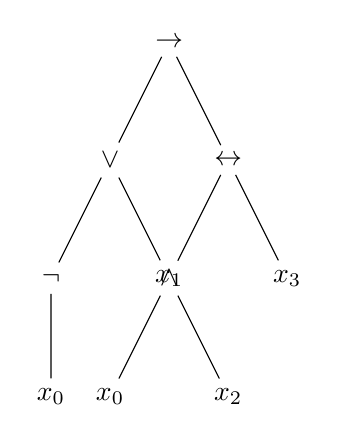
\begin{tikzpicture}
        \node {$\to$}
        child { node {$\lor$}
          child { node {$\lnot$} child { node {$x_0$} } }
          child { node {$x_1$} }
        }
        child { node {$\leftrightarrow$}
          child {
            node {$\land$}
            child { node {$x_0$} }
            child { node {$x_2$} }
          }
          child { node {$x_3$} }
        }
        ;
      \end{tikzpicture}
    \end{figure}
  \end{exm}

  \section{Sémantique.}
  
  \begin{lem}
    Soit $\nu$ une fonction de $\mathcal{P}$ dans $\{0,1\}$ appelé \textit{valuation}.
    Alors $\nu$ s'étend de manière unique en une fonction $\bar{\nu}$ de $\mathcal{F}$ dans $\{0,1\}$ telle que 
    \begin{itemize}
      \item sur $\mathcal{P}$, $\nu = \bar{\nu}$ ;
      \item si $F, G \in \mathcal{F}$ sont des formules alors 
        \begin{itemize}
          \item $\bar{\nu}(\lnot F) = 1 - \bar{\nu}(F)$ ;
          \item $\bar{\nu}(F \lor G) = 1$ ssi $\bar{\nu}(F) = 1$ ou\footnote{C'est un "ou" inclusif : on peut avoir les deux (ce qui est très différent du "ou" exclusif dans la langue française).} $\bar{\nu}(G) = 1$ ;
          \item $\bar{\nu}(F \land G) = \bar{\nu}(F) \times \bar{\nu}(G)$ ;
          \item $\bar{\nu}(F \to G) = 1$ ssi $\bar{\nu}(G) = 1$ ou $\bar{\nu}(F) = 0$ ;
          \item $\bar{\nu}(F \leftrightarrow G) = 1$ ssi $\bar{\nu}(F) = \bar{\nu}(G)$.
        \end{itemize}
    \end{itemize}
    Par abus de notations, on notera $\nu$ pour $\bar{\nu}$ par la suite.
  \end{lem}
  \begin{prv}[Idée de preuve]
    \begin{description}
      \item[Existence.]
        On définit en utilisant le lemme de lecture unique, et par induction sur $\mathcal{F}$ :
        \begin{itemize}
          \item $\bar{\nu}$ est définie sur $\mathcal{F}_0 = \mathcal{P}$ ;
          \item si $\bar{\nu}$ est définie sur $\mathcal{F}_n$ alors pour $F \in \mathcal{F}_{n+1}$, on a la disjonction de cas
            \begin{itemize}
              \item si $F = \lnot G$ avec $G \in \mathcal{F}_n$, et on définit $\bar{\nu}(F) = 1 - \bar{\nu}(F_1)$ ;
              \item \textit{etc} pour les autres cas.
            \end{itemize}
        \end{itemize}
      \item[Unicité.]
        On montre que si $\lambda = \nu$ sur $\mathcal{P}$ alors $\bar{\lambda} = \bar{\nu}$ si $\bar{\lambda}$ et $\nu$ vérifient les égalités précédents.
    \end{description}
  \end{prv}

  \begin{exm}[Table de vérité]
    Pour la formule \[F = \verb|((|x_1\to x_2\verb|)| \to \verb|(|x_2 \to x_1\verb|))|, \] on construit la table 
    \begin{table}[H]
      \centering
      \begin{tabular}{r|cccc}
        $x_1$ & 0 & 0 & 1 & 1\\ \hline
        $x_2$ & 0 & 1 & 0 & 1\\ \hline
        $x_1 \to x_2$ & 1 & 1 & 0 & 1\\ \hline
        $x_2 \to x_1$ & 1 & 0 & 1 & 1\\ \hline
        $F$ & 1 & 0 & 1 & 1
      \end{tabular}
    \end{table}
  \end{exm}

  \begin{defn}
    \begin{itemize}
      \item Une formule $F$ est dite \textit{satisfaite par une valuation $\nu$} si  $\nu(F) = 1$.
      \item Une \textit{tautologie} est une formule satisfaite pour toutes les valuations.
      \item Un ensemble $\mathcal{E}$ de formules est \textit{satisfiable} s'il existe une valuation qui satisfait toutes les formules de $\mathcal{E}$.
      \item Un ensemble $\mathcal{E}$ de formules est \textit{finiment satisfiable} si tout sous-ensemble fini de $\mathcal{E}$ est satisfiable.
      \item Une formule $F est \mathit{conséquence sémantique}$ d'un ensemble de formules $\mathcal{E}$ si toute valuation qui satisfait $\mathcal{E}$ satisfait $F$.
      \item Un ensemble de formules $\mathcal{E}$ est \textit{contradictoire} s'il n'est pas satisfiable.
      \item Un ensemble de formules $\mathcal{E}$ est \textit{finiment contradictoire} s'il existe un sous-ensemble fini contradictoire de $\mathcal{E}$.
    \end{itemize}
  \end{defn}

  \begin{thm}[compacité du calcul propositionnel]
    \label{chap1-comp}
    On donne trois énoncés équivalents (équivalence des trois énoncés laissé en exercice) du théorème de compacité du calcul propositionnel.

    \begin{description}
      \item[Version 1.] Un ensemble de formules $\mathcal{E}$ est satisfiable si et seulement s'il est finiment satisfiable.
      \item[Version 2.] Un ensemble de formules $\mathcal{E}$ est contradictoire si et seulement s'il est finiment contradictoire.
      \item[Version 3.] Pour tout ensemble $\mathcal{E}$ de formules du calcul propositionnel, et toute formule $F$, $F$ est conséquence sémantique de $\mathcal{E}$ si et seulement si $F$ est conséquence sémantique d'un sous-ensemble fini de $\mathcal{E}$.
    \end{description}
  \end{thm}
  \begin{prv}
    Dans le cas où $\mathcal{P} = \{x_0, x_1, \ldots\} $ est au plus dénombrable (le cas non dénombrable sera traité après).
    On démontre le cas "difficile" de la version 1 (\textit{i.e.} finiment satisfiable implique satisfiable).
    Soit $\mathcal{E}$ un ensemble de formules finiment satisfiable.
    On construit par récurrence une valuation $\nu$ qui satisfasse  $\mathcal{E}$ par récurrence : on construit $\varepsilon_0, \ldots, \varepsilon_n, \ldots$ tels que $\nu(x_0) = \varepsilon_0, \ldots, \nu(x_n) = \varepsilon_n, \ldots$
    \begin{itemize}
      \item Cas de base.
        On définit la valeur de $\varepsilon_n$ pour $x_0 \in \mathcal{P}$.
        \begin{enumerate}
          \item soit, pour tout sous-ensemble fini $B$ de $\mathcal{E}$, il existe une valuation $\lambda$ qui satisfait $B$ avec $\lambda(x_0) = 0$ ; \label{chap1-comp-cas1}
          \item soit, il existe un sous-ensemble fini $B_0$ de $\mathcal{E}$, pour toute valuation $\lambda$ qui satisfait $B_0$, on a $\lambda(x_0) = 1$.  \label{chap1-comp-cas2}
        \end{enumerate}

        Si on est dans le cas~\ref{chap1-comp-cas1}, on pose $\varepsilon_0 = 0$, et sinon (cas~\ref{chap1-comp-cas2}) on pose $\varepsilon_0 = 1$.
      \item Cas de récurrence.
        On montre, par récurrence sur $n$, la propriété suivante :
        \begin{quote}
          il existe une suite $\varepsilon_0, \ldots, \varepsilon_n$ (que l'on étend, la suite ne change pas en fonction de $n$) de booléens telle que, pour tout sous-ensemble fini $B$ de $\mathcal{E}$, il existe une valuation $\nu$ satisfaisant  $B$ et telle que $\nu(x_0) = \varepsilon_0$, \ldots, et $\nu(x_n) = \varepsilon_n$.
        \end{quote}
        \begin{itemize}
          \item Pour $n = 0$, soit on est dans le cas~\ref{chap1-comp-cas1}, et on prend $\varepsilon_0 = 0$ et on a la propriété ; soit on est dans le cas~\ref{chap1-comp-cas2};, et on prend $B$ un sous-ensemble fini de $\mathcal{E}$, alors $B \cup B_0$ est un ensemble fini donc satisfiable par une valuation $\nu$. La valuation satisfait  $B_0$ donc  $\nu(x_0) = 1$ et $\nu$ satisfait $B$.
            On a donc la propriété au rang $0$.
          \item Hérédité.
            Par hypothèse de récurrence, on a une suite $\varepsilon_0, \ldots, \varepsilon_n$.
            \begin{enumerate}
              \item Soit, pour tout sous-ensemble fini $B$ de $\mathcal{E}$, il existe $\nu$ qui satisfait $B$ et telle que $\nu(x_0) = \varepsilon_0$,  \ldots, $\nu(x_n) = \varepsilon_n$, et  $\nu(x_{n+1}) = 0$. On pose $\varepsilon_{n+1} = 0$.
              \item Soit il existe $B_{n+1}$ un sous-ensemble fini de $\mathcal{E}$ tel que, pour toute valuation $\nu$ telle que $\nu$ satisfait $B_{n+1}$ et $\nu(x_0) = \varepsilon_0, \ldots, \nu(x_n) = \varepsilon_n$, on a $\nu(x_{n+1}) = 1$ et on pose $\varepsilon_{n+1} = 1$.
            \end{enumerate}
            Montrons l'hérédité :
            \begin{enumerate}
              \item vrai par définition ;
              \item soit $B$ un sous-ensemble fini de $\mathcal{E}$. On considère $B \cup B_{n+1}$, soit $\nu$ telle que  $\nu(x_0) = \varepsilon_0$, \ldots, $\nu(x_n) = \varepsilon_n$.
                On a que $\nu$ satisfait $B_{n+1}$ donc $\nu(x_{n+1}) = 1 = \varepsilon_{n+1}$ et $\nu$ satisfait $B$.
            \end{enumerate}
        \end{itemize}
        On a donc la propriété pour tout $n$.
    \end{itemize}
    Finalement, soit $\delta$ une valuation telle que, pour tout $i$, $\delta(x_i) = \varepsilon_i$.
    Montrons que  $\delta$ satisfait  $\mathcal{E}$.
    Soit $F \in \mathcal{E}$.
    On sait que $F$ est un mot (fini), donc contient un ensemble fini de variables inclus dans $\{x_0, \ldots, x_n\}$.
    D'après la propriété par récurrence au rang $n$, il existe une valuation $\nu$
    qui satisfait  $F$ et telle que $\nu(x_0) = \varepsilon_0, \ldots, \nu(x_n) = \varepsilon_n$, et donc  $\nu$ et $\delta$ coïncident sur les variables de $F$.
    Donc (lemme simple), elles coïncident sur toutes les formules qui n'utilisent que ces variables.
    Donc, $\delta(F) = 1$, et on en conclut que  $\delta$ satisfait $\mathcal{E}$.
  \end{prv}

  Dans le cas non-dénombrable, on utilise le \textit{lemme de Zorn}, un équivalent de l'\textit{axiome du choix}.

  \begin{defn}
    Un ensemble ordonné $(X, \mathcal{R})$ est inductif si pour tout sous-ensemble $Y$ de $X$ totalement ordonné par $\mathcal{R}$ (\textit{i.e.} une chaîne) admet un majorant dans $X$.
  \end{defn}

  \begin{rmk}
    On considère ici un majorant et non un plus grand élément (un maximum).
  \end{rmk}

  \begin{exm}
    \begin{enumerate}
      \item Dans le cas $(\mathcal{P}(X), \subseteq )$, le majorant est l'union des parties de la chaîne, il est donc inductif.
      \item Dans le cas $(\mathds{R}, \le)$, il n'est pas inductif car $\mathds{R}$ n'a pas de majorant dans $\mathds{R}$.
    \end{enumerate}
  \end{exm}

  \begin{lem}[Lemme de Zorn]
    Si $(X, \mathcal{R})$ est un ensemble ordonné inductif non-vide, il admet au moins un élément maximal.
  \end{lem}

  \begin{rmk}
    Un élément maximal n'est pas nécessairement le plus grand.
  \end{rmk}

  \vspace{1.5em}

  \begin{prv}[Cas non-dénombrable pour le théorème~\ref{chap01-comp}]
    Soit $\mathcal{E}$ un ensemble de formules finiment satisfiable, et $\mathcal{P}$ un ensemble de variables.
    On note $\mathcal{V}$ l'ensemble des valuations partielles prolongeables pour toute partie finie $\mathcal{C}$ de $\mathcal{E}$ en une valuation satisfaisant $\mathcal{C}$.
    C'est-à-dire :
    {
      \footnotesize
    \[
    \mathcal{V} := \mleft\{\,\varphi \in \bigcup_{X \subseteq \mathcal{P}} \{0,1\}^X \;\middle|\; \forall \mathcal{C} \in \wp_\mathrm{f}(\mathcal{E}), \exists \delta \in \{0,1\}^\mathcal{P}, 
      \begin{array}{l}
        \delta_{|\mathrm{dom}(\varphi)} = \varphi\\
        \forall F \in \mathcal{C}, \delta(F) = 1
      \end{array}
    \,\mright\} 
    .\] 
    }

    L'ensemble $\mathcal{V}$ est non-vide car contient l'application vide de $\{0,1\}^\emptyset$ car $\mathcal{E}$ est finiment satisfiable.
    On défini la relation d'ordre~$\preceq$ sur  $\mathcal{V}$ par : \[
      \varphi \preceq \psi \quad \text{ ssi } \quad \psi \text{ prolonge } \varphi
    .\]
    Montrons que $(\mathcal{V}, \preceq)$ est inductif.
    Soit $\mathcal{C}$ une chaîne de $\mathcal{V}$et construisons un majorant de $\mathcal{C}$.
    Soit $\lambda$ la valuation partielle définie sur $\operatorname{dom}\lambda = \bigcup_{\varphi \in \mathcal{C}} \operatorname{dom} \varphi$, par : 
    si $x_i \in \operatorname{dom} \lambda$ alors il existe $\varphi \in \mathcal{C}$ tel que $x_i \in \operatorname{dom} \varphi$ et on pose $\lambda(x_i) = \varphi(x_i)$.

    La valuation $\lambda$ est définie de manière unique,  \textit{i.e.} ne dépend pas du choix de $\varphi$. En effet, si $\varphi \in \mathcal{C}$ et $\psi \in \mathcal{C}$, avec $x_i \in \operatorname{dom} \varphi \cap \operatorname{dom} \psi$, alors on a $\varphi \preceq \psi$ ou $\psi \preceq \varphi$, donc $\varphi(x_i) = \psi(x_i)$.

    Autrement dit, $\lambda$ est la limite de $\mathcal{C}$.
    Montrons que $\lambda \in \mathcal{V}$.
    Soit $B$ une partie finie de $\mathcal{E}$. On cherche $\mu$ qui prolonge $\lambda$ et satisfait $B$.
    L'ensemble de formules $B$ est fini, donc utilise un ensemble fini de variables, dont un sous-ensemble fini $\{x_{i_1}, \ldots, x_{i_n}\} \subseteq \operatorname{dom}(\lambda)$.
    Il existe $\varphi_1, \ldots, \varphi_n$ dans $\mathcal{C}$ telle que $x_{i_1} \in \operatorname{dom} \varphi_1, \ldots, x_{i_n} \in \operatorname{dom} \varphi_n$.
    Comme $\mathcal{C}$ est une chaîne, donc soit $\varphi_0 = \max_{i \in \llbracket 1,n\rrbracket} \varphi_i$ et on a $\varphi_0 \in \mathcal{C}$.
    On a, de plus, $x_{i_1}, \ldots, x_{i_n} \in \operatorname{dom}(\varphi_0)$.
    Soit $\varphi_0 \in \mathcal{V}$ prolongeable en $\psi_0$ qui satisfait $B$.
    On définit :
    \begin{align*}
      \mu: \mathcal{P} &\longrightarrow \{0,1\}  \\
      x \in \operatorname{dom} \lambda &\longmapsto \lambda(x) \\
      x \in \operatorname{var} B &\longmapsto \psi_0(x) \\
      \text{sinon} &\longmapsto 0
    .\end{align*}

    On vérifie que la définition est cohérente sur l'intersection car $\lambda$ et $\psi_0$ prolongent tous les deux $\varphi_0$ et donc  $\lambda \in \mathcal{V}$ d'où $\mathcal{V}$ est inductif.

    Suite la preuve plus tard.
  \end{prv}

\end{document}
